
\section{Question 2}
\label{part2}
Write a Python program that:
\begin{itemize} 
\item Uses ``Carbon Date'' to estimate the age of each links(s) in a tweet
		-See:``http://ws-dl.blogspot.com/2013/04/2013-04-19-carbon-dating-web.html''
\item Create a histogram of (Age\textsubscript{tweet} - Age\textsubscript{link})
	    .Many (most?) deltas will be 0,but there should be many>0
\item For these, compute: median, mean, std dev, std err 


\item Use wget to download the text for all the links. Hold on to those,
		 we'll come back to them later.
		 -See :
		 	   ``\url{http://superuser.com/questions/55040/save-a-single-web-page-with-background-images-with-wget}''
		 	   ``\url{http://stackoverflow.com/questions/6348289/download-a-working-local-copy-of-a-webpage}''
\end{itemize}

\subsection{Solution}
\begin{itemize}
\item Carbon Date tool installed as per instructions provided in readme file.
\item Few URI's were consuming lot of time to query all of its services .So,I have divided 10000 URI's to 10 files and ran 
	  10 scripts on different linux servers. 
\item Few changes are made to local.py from the carbon tool in order to read 1000 URI's from a text file and write back the result into
	  an other text file in json format. 
\item To find an age of a link, I have written a python program (calculateDays.py) which will take the date and return days. 
\item Mean,Median and standard deviation are calculated using statistics python package.
\end{itemize}

\subsection{Code Listing}
\subsubsection{local.py}
\lstinputlisting[language=Python,breaklines = true,frame=single,caption={Python program for getting creation date for URI's}, label=lst:q2-1,captionpos=b,numbers=left,showspaces=false,showstringspaces=false,basicstyle=\footnotesize]{local.py}
\newpage
\subsubsection{CalculateDays.py}
\lstinputlisting[language=Python,breaklines = true,frame=single,caption={Python program for calculating the age of URI's}, label=lst:q2-2,captionpos=b,numbers=left,showspaces=false,showstringspaces=false,basicstyle=\footnotesize]{calculateDays.py}
\subsubsection{StatusCodesHistogram.py}
\lstinputlisting[language=Python,breaklines = true,frame=single,caption={R program for creating histogram of Tweet Age - Link Age}, label=lst:q1-2,captionpos=b,numbers=left,showspaces=false,showstringspaces=false,basicstyle=\footnotesize]{StatusCodesHistogram.R}
\newpage
\subsection{Results}

\lstinputlisting[language=Python,breaklines = true,frame=single,caption={Sample Result for Above Program}, label=lst:q1-1,captionpos=b,numbers=none,showspaces=false,showstringspaces=false,basicstyle=\footnotesize]{CarbonDateSampleOutput.txt}

\newpage


\begin{figure}[ht]    
    \begin{center}
        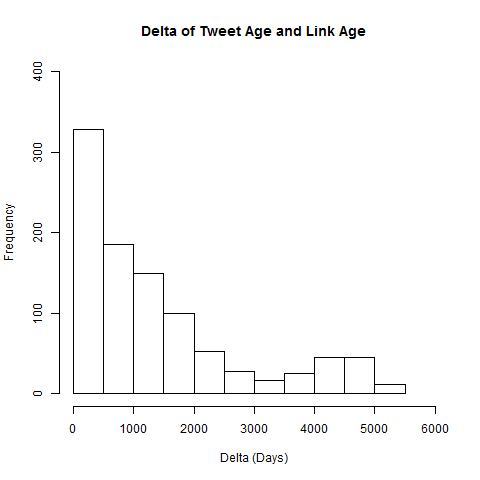
\includegraphics[scale=0.60]{DeltaHistogram.png}
        \caption{Histogram}
        \label{RedirectHistogram}
    \end{center}
\end{figure}


